%\lipsum[21-40]

%\nocite{Lax1956,Cooley1965,Banach1924}

Self-assembly is a class of formation process in which a product is constructed without explicit manipulation of its individual parts: many---often identical---parts come together by utilizing the dynamics of their environment to create the finished structure. Such processes can often be encouraged by manipulating broadly controlled parameters of the assembly environment such as temperature, solution content, and assembly subunit selection. 

There are many examples of both natural and synthetic self-assembly process that take a wide variety of length scales and serve a plethora of functions. An area of much active research is the self-assembly of RNA, proteins, and viral capsids. These biological processes act on the nano scale and, while it is known that their formation can be aided by a variety of secondary mechanisms, the formation process is not well understood in general. Synthetic examples of molecular self assembly include the formation of supramolecular cages. These cages, composed of many subunit molecules, are large enough to encapsulate smaller molecules and show promise in contributing to a number of medical and scientific fields including drug delivery and nano-scale circuits. 

In general, the processes of biological self-assembly are not well understood due to difficulties arising from their small length scale. Conversely, synthetic self-assembly processes often lack the complexity and sophistication of their biological equivalents. In both cases, central themes of self-assembly are similar. Of primary importance is identifying the pathways of formation which consist of a specific order in which unfinished intermediate states are visited before the assembly is completed. It is thought that these pathways are often robust in the sense that the process follows a very small number of pathways to form the end product, despite an overwhelmingly large number of distinct pathways that are possible. Also of interest is identifying mechanisms by which failed or flawed formations can be avoided or minimized. Possible strategies include the selection of specific precursors, the selection of solution, and the mid-assembly control of experimental parameters. 

The goal of this work is to provide a framework in which the interplay between the combinatorial and geometric aspects of self-assembly processes can be analyzed. 

\section{Polyhedra}

We focus on the self-assembly of polyhedral structures for a number of reasons. First, there is a rich history of using polyhedra as representative models for molecular structure~\cite{Sachse1890}. Whether it is treating carbon atoms like tetrahedra or the $C_{60}$ Buckminsterfullerene as a truncated icosahedron, it is natural to model spherical meshes of molecules as polyhedra~\cite{Kroto1985}. One could view each molecular subunit (carbon atom in the case of $C_{60}$) as a vertex and each subunit to subunit bond as an edge to define the structure as a polyhedron. Sometimes the dual perspective--with each subunit being a polyhedral face and edges existing between bonded subunits--is more useful. 

Aside from the clear connection to molecular structure, polyhedra are also mathematical objects with a rich literature and known properties. First by the ancient Greeks, polyhedra are ubiquitous in everyday culture: whether it be in architecture, computer graphics, or board games. As three dimensional structures composed of two-dimensional faces, the construction and assembly of polyhedra is easier and more reliable than other three dimensional alternatives. 

There are a few canonical classes of polyhedra we consider throughout this work. The Platonic solids, composed of the tetrahedron, cube, octahedron, dodecahedron, and icosahedron are the five polyhedra that are composed of only one type of regular polygon. The tetrahedron is self-dual with the cube-octahedron and dodecahedron-icosahedron pairs dual to each other. By relaxing the condition to allow the polyhedra to be composed of two or more regular polygons, the Archimedean solids are defined. With a total of thirteen member polyhedra, the Archimedean solids also have the property that each vertex has identical connectivity properties. Dual to the Archimedean solids are the Catalan solids. Also composed of 13 polyhedra, each Catalan solid has only one type of face, but that polygon is not regular~\cite{Cromwell1997}.

The theory of polytopes provides a $d$-dimensional generalization of polyhedra. While we restrict our focus to $3$-dimensional polytopes, the mathematical structure of polytope theory is at times useful. In particular, a $0$-dimensional polytope is a point, a $1$-dimensional polytope is an edge, a $2$-dimensional polytope is a polygon and a $3$-dimensional polytope is a polyhedron. A polyhedron along with all of its $0$, $1$, and $2$-dimensional substructures is called a polytopal complex~\cite{Ziegler1995}.

\section{Scientific Motivation}

As presented below, polyhedra play in important role in many organic and synthetic self-assembly processes. From being a model for molecular subunits to representing an assembled spherical product, polyhedra form a natural construct for describing a variety of these processes. We present a number of motivating scientific applications that demonstrate the interplay between polyhedra and self-assembly~\cite{Kaplan2014}.

\subsection{Self-Folding Polyhedra}
\label{ssc:SelfFold}
In experiment, Pandey et al. have been able to form closed sub-millimeter scale polyhedral structures from the self-folding of flat polyhedral nets~\cite{Pandey2011}. Using photolithography, these nets are cut from a two dimensional sheet with great precision. By adding a specific amount of solder at the net's hinges, surface tension from the melted solder causes the net to fold up into the closed polyhedron. Several different polyhedra have been attempted with varying degrees of success. It has been argued that the geometric structure of the polyhedron are largely determinant of the net's propensity to successfully assemble into the polyhedron. In some cases, two distinct polyhedral isomers can be formed from the same net~\cite{Pandey2014}.

\subsection{Molecular Cages}

Self-assembly of molecular cages are the subject of much active research. By isolating individual molecules of interest inside a molecular cage, targeted application of these molecules is theoretically possible. This has enormous implications in the medical industry. Additionally, by creating a grid-like network of such cages, it may be possible to construct functional electric circuitry on the nano scale~\cite{Sun2010}. 

Fujita et. al. have theorized and subsequently synthesized a family of organometallic cages consisting of metallic connector molecules (M) that each connect four bent ligand molecules (L). With the M molecules as vertices and the L molecules as edges, they can form polyhedral cages. Due to geometric constraints, the number of M and L molecules in  a completed cage must satisfy  $|M| = k$ and $|L| = 2k$ for $k \in 6, 12, 24, 30, 60$. Each of these five choice of $k$ results in a cage that geometrically resembles a specific Archemedian solid~\cite{Li2011}. 

In one experiment, two different ligands ($L_1$ and $L_2$) with slightly different bend angles were used. As the ratio of $L_1:L_2$ was varied, each ratio only resulted in the formation of one of the possible cages. More specifically, for ratios $L_1:L_2 < 0.25$ only $M_{12}L_{24}$ formed and for  $L_1:L_2 > 0.25$ only $M_{24}L_{48}$ was formed. Explanation for this steep and curious cutoff remains an open problem that mathematical approaches could shed light on.

In experiments by Liu et al, polyhedral supramolecular cages made from different molecular species were synthesized~\cite{Liu2011}. Theoretically, a tiling pattern of the molecular species is chemically possible, but it was not observed experimentally. Additional experiments in which copies of two types of molecular species could be combined to form two different polyhedral cages were proposed. It is unknown if both potential polyhedral cages would form or if one would be significantly more favorable over the other. Being able to predict the results of such experiments via mathematical analysis and simulation would be a significant contribution toward optimizing strategies for the self-assembly of supramolecular cages. 

\subsection{Viral Capsid Assembly}

With forces such as friction playing a much bigger role on their length scale, biological viruses are remarkable at robustly replicating themselves. While this topic has been well studied and a wide variety of mechanisms have been evidenced to contribute, there still is no general understanding of the process in which a virus' capsid is formed~\cite{Berger1994}. Viral capsids come in many shapes and sizes, but a significant portion of them are icosahedral in structure. The seminal work of Caspar and Klug identified this connection between polyhedra and viral capsids, and continues to inform research on the process in which they are formed~\cite{Caspar1962}. Understanding the pathways by which a viral capsid forms may be key in preventing or slowing down replication in future medical research.  

\subsection{RNA and Protein Folding}

Protein and RNA folding are active fields of research. If we can predict the three dimensional structure of a RNA or protein based on its amino acid sequence, we will know more about its biological function. As many human and animal disorders are caused by proteins folding abnormally, their cures may lie in the understanding of the folding pathway. While we do not directly consider applications relating to RNA and protein folding, success with the above problems may also provide insights for this complex topic~\cite{Lindorff-Larsen2011}.


\section{Mathematical Constructs for Self-Assembly}

A common theme for mathematically modeling self-assembly involves specifying a framework of rules or steps by which the self-assembly of a particular structure can occur. Given such a model, all of the possible intermediate stages or states in which the process can occupy is enumerated. With this atlas of possible configurations represented as a graph, the entire self-assembly process can be described as a path through this graph. Using the mathematical structure of the graph, a quantitative analysis of the process is possible. The following are different mathematical approaches to self assembly. Some follow the graph enumeration approach, but others are more qualitative. 

%The concept of formation pathways that occur with overwhelming frequency relative to the myriad of other theoretically possible pathways is a primary interest of our work. To identify the nature of such dominant pathways is to identify the mechanism of self-assembly itself. This knowledge would hopefully enable the proliferation of the self-assembled products to become more efficient and faster, or in cases such as biological viruses, inhibit formation altogether. There are several means, both quantitative and qualitative, by which we seek to identify and study these dominant pathways. 

\subsection{Attachment}

First proposed by Wales, the Building Game is a discrete attachment model that simulates the sequential construction of polyhedral structures~\cite{Wales1987}. Subsequent work by Zlotnick modified the original model and used it to examine icosahedral viral capsid assembly~\cite{Zlotnick1994, Endres2005}. Much of our work revolves around the Building Game and it is explained in great depth in the next chapter.

%By modeling the construction of an icosahedron as a face by face    

%--More!

%
% The Building Game (BG) for a polyhedron $\mathcal{P}$ begins with a single face of $\mathcal{P}$ and iteratively attaches faces to the existing partially formed polyhedron until all faces of $\mathcal{P}$ are present. We denote the set of $\mathcal{P}$'s faces, edges, and vertices as $F(\mathcal{P}),E(\mathcal{P}),$ and $V(\mathcal{P})$ respectively. A Building Game \textbf{pathway} is a linear ordering $f_1,f_2,f_3,\ldots,f_N$ of the faces of $\mathcal{P}$ such that for $j = 2,\ldots,N$ there exists edges $e_1,e_2,\ldots,e_k \in E(\mathcal{P})$ with  $k \geq 1$ satisfying
%$$\left(e_1\cup\cdots\cup e_k \right)\subset \left(f_j\cap\left(\bigcup_{i=1}^{j-1}f_i\right)\right)$$
%Since the order and location of attachment in the Building Game can vary, many partially formed polyhedra, called \textbf{intermediates}, are possible. Each intermediate $x$ can be represented as $x = \cup_{i=1}^tf_i$ where $f_1,\ldots,f_t,\ldots,f_N$ is a BG pathway. For a given polyhedron, we are interested in enumerating all of the distinct intermediates up to rotational equivalence. The  \textbf{attachment sites} of an intermediate $x$ are the set of faces $\{f_k\}$ such that $f_k\cap x = e_1\cup e_2 \cup \cdots$ for some edges $e_1,e_2,\ldots \in E(\mathcal{P})$. In other words, the attachment sites are the places in which a new face may join $x$ as part of a valid BG pathway.
%
%\begin{figure}[!h]
%%\centering
%%\includegraphics[width=0.8\textwidth]{bg.png}
%\caption{Dodecahedron Building Game example.}
%\label{fig:bg}
%\end{figure}
%
%The \textbf{state space} for a particular polyhedron $\mathcal{P}$ is a graph that represents the space of all distinct intermediates and the BG pathways for $\mathcal{P}$. Each node of the state space represents a single intermediate and a connection exists between two nodes if it is possible to construct one of the corresponding intermediates by adding a single face to the other. Each path through the state space, starting at an intermediate with one face and ending at the intermediate with all faces, represents one of the polyhedron's BG pathways. 
%
%\begin{figure}[h]
%%\centering
%%\includegraphics[width=0.8\textwidth]{cube_bg.png}
%\caption{The state space of the cube.}
%\label{fig:cube_bg}
%\end{figure}
%
%
%%\begin{figure}[h]
%%\centering
%%\includegraphics[width=0.8\textwidth]{dodecahedronSS.png}
%%\caption{Configuration space of the dodecahedron}
%%\label{fig:dodecahedronSS}
%%\end{figure}
%
%
%For a state space edge going between an intermediate with $k$ faces to one with $k+1$ faces, the \textbf{degeneracy number} is the number of different attachment sites on the $k$-faced intermediate that will produce the $k+1$-faced intermediate. For example, the state space edge between the cube intermediate with 1 face and the intermediate with 2 faces has degeneracy number 4 since each of the first square's four edges will form the same intermediate when a second square is attached. 
%
%
%As we consider polyhedra with more and more faces, there is a combinatorial explosion in the number intermediates in state space. While the 6-faced cube state space has only 8 vertices and 9 edges, the 20-faced icosahedron state space has 2,649 vertices and 17,241 edges and the 26-faced truncated cuboctahedron state space has 1,525,605 vertices and 17,672,377. We have computed the BG state space for all polyhedra in the Platonic, Archimedean, and Catalan solid classes of up to 30 faces. Due to computational constraints, we do not compute the BG state space for larger polyhedra, but we are exploring the possibility of non-enumerative exploration of the state space of large polyhedra in the future. 
%
%The Building Game suffers from the fact that it only allows one end product to form and cannot model physically realistic formation errors. However its simplicity is a feature that aids analysis. We discuss models that do capture formation errors below.  
%
%
\subsection{Folding}
Another model--we refer to as the Folding Model--was used to model the self-folding of meso-scale metallic polyhedra mentioned in section~\ref{ssc:SelfFold}. In this model, a polyhedron's net is sequentially folded up into the finished polyhedron. At each stage one vertex is closed to form a pyramidal structure by a folding move. In analogy with the Building Game, we can define folding intermediates to be partially folded states and a state spaces where intermediates are connected if one can form the other with a single fold. One possible sequence of fold resulting in the octahedron is shown in figure~\ref{fig:fold_octa}. 

Interestingly, each polyhedron may has multiple nets. In fact, the number of distinct nets grows rapidly with the size of the polyhedron. Certain nets have different folding pathways and measuring the favorability of one of these nets over another introduces an design problem. If nets that fold into the completed polyhedron most reliably can be identified, the efficiency of the self-assembly process can be optimized~\cite{Pandey2011, Pandey2014}

\begin{figure}[h]

       \centering
                
\includegraphics[width=0.18\textwidth]{images/folds_0.eps}
                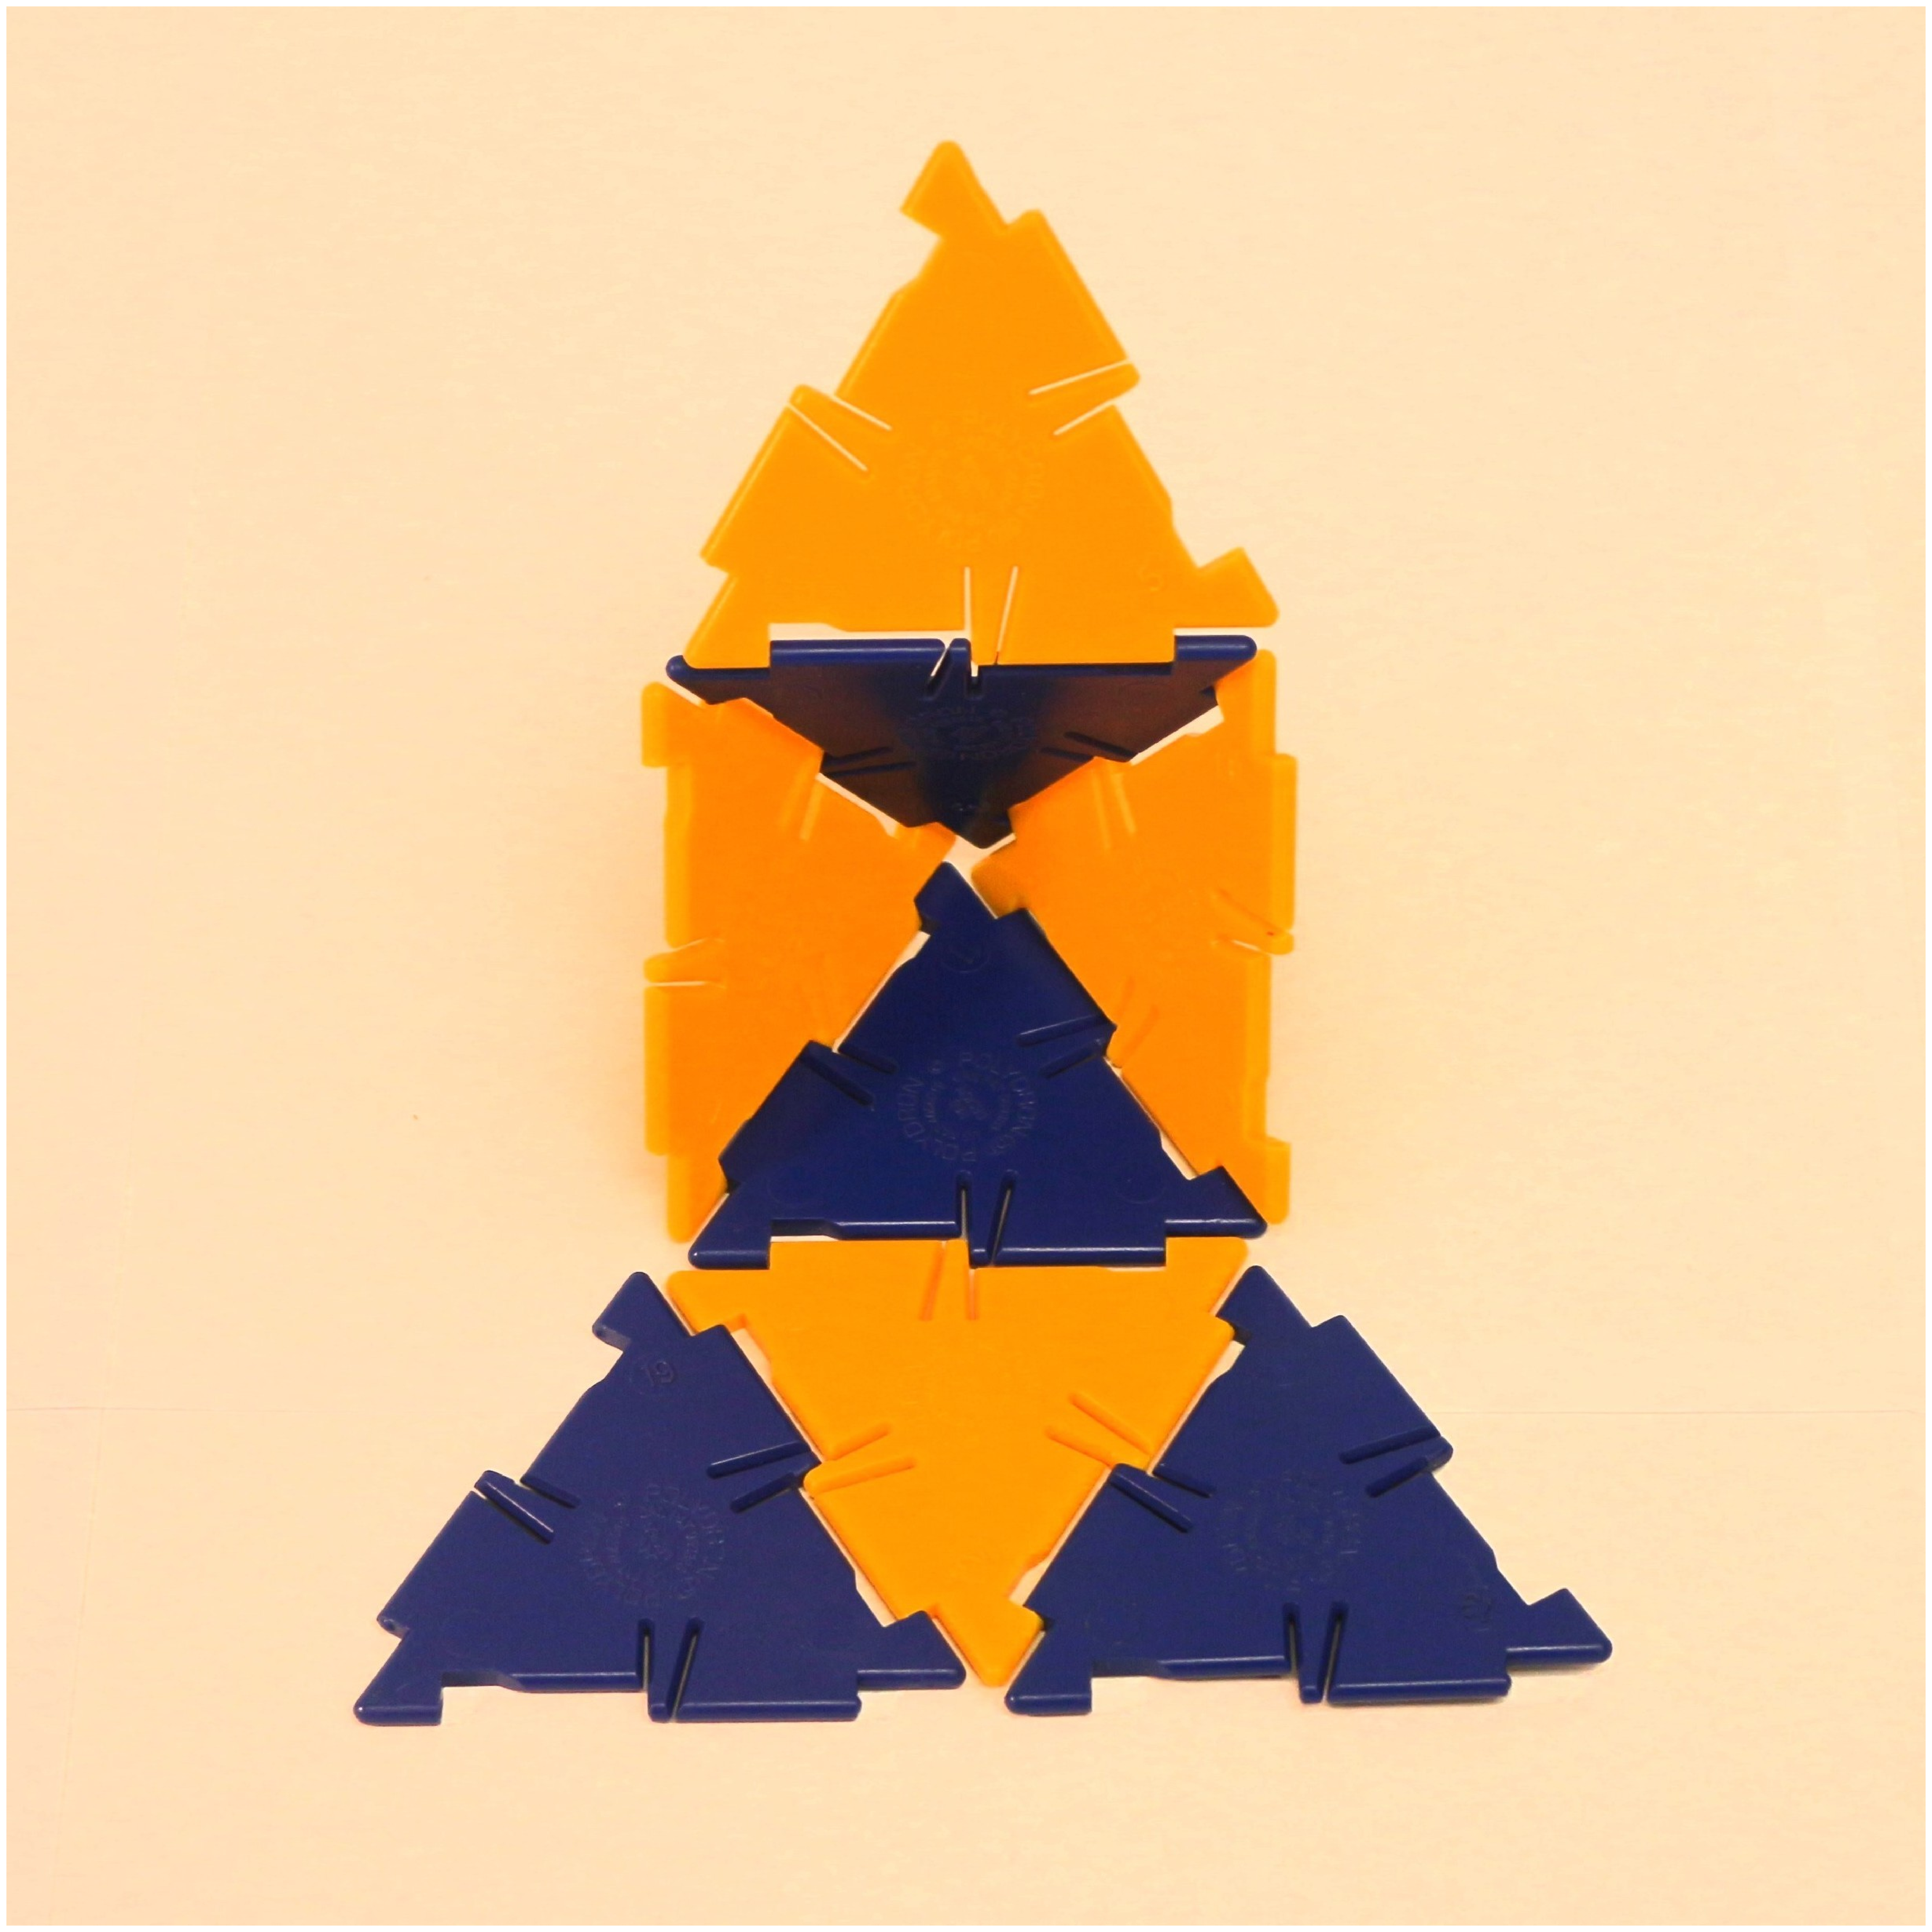
\includegraphics[width=0.18\textwidth]{images/folds_1.eps}
                
\includegraphics[width=0.18\textwidth]{images/folds_2.eps}
                
\includegraphics[width=0.18\textwidth]{images/folds_3A.eps}
                
\includegraphics[width=0.18\textwidth]{images/folds_4A.eps}

\caption{A sequence of Folding Model intermediates beginning with an octahedron net and successfully forming an octahedron.}
\label{fig:fold_octa}
\end{figure}

\begin{figure}[h]

       \centering

                
\includegraphics[width=0.18\textwidth]{images/folds_0.eps}
                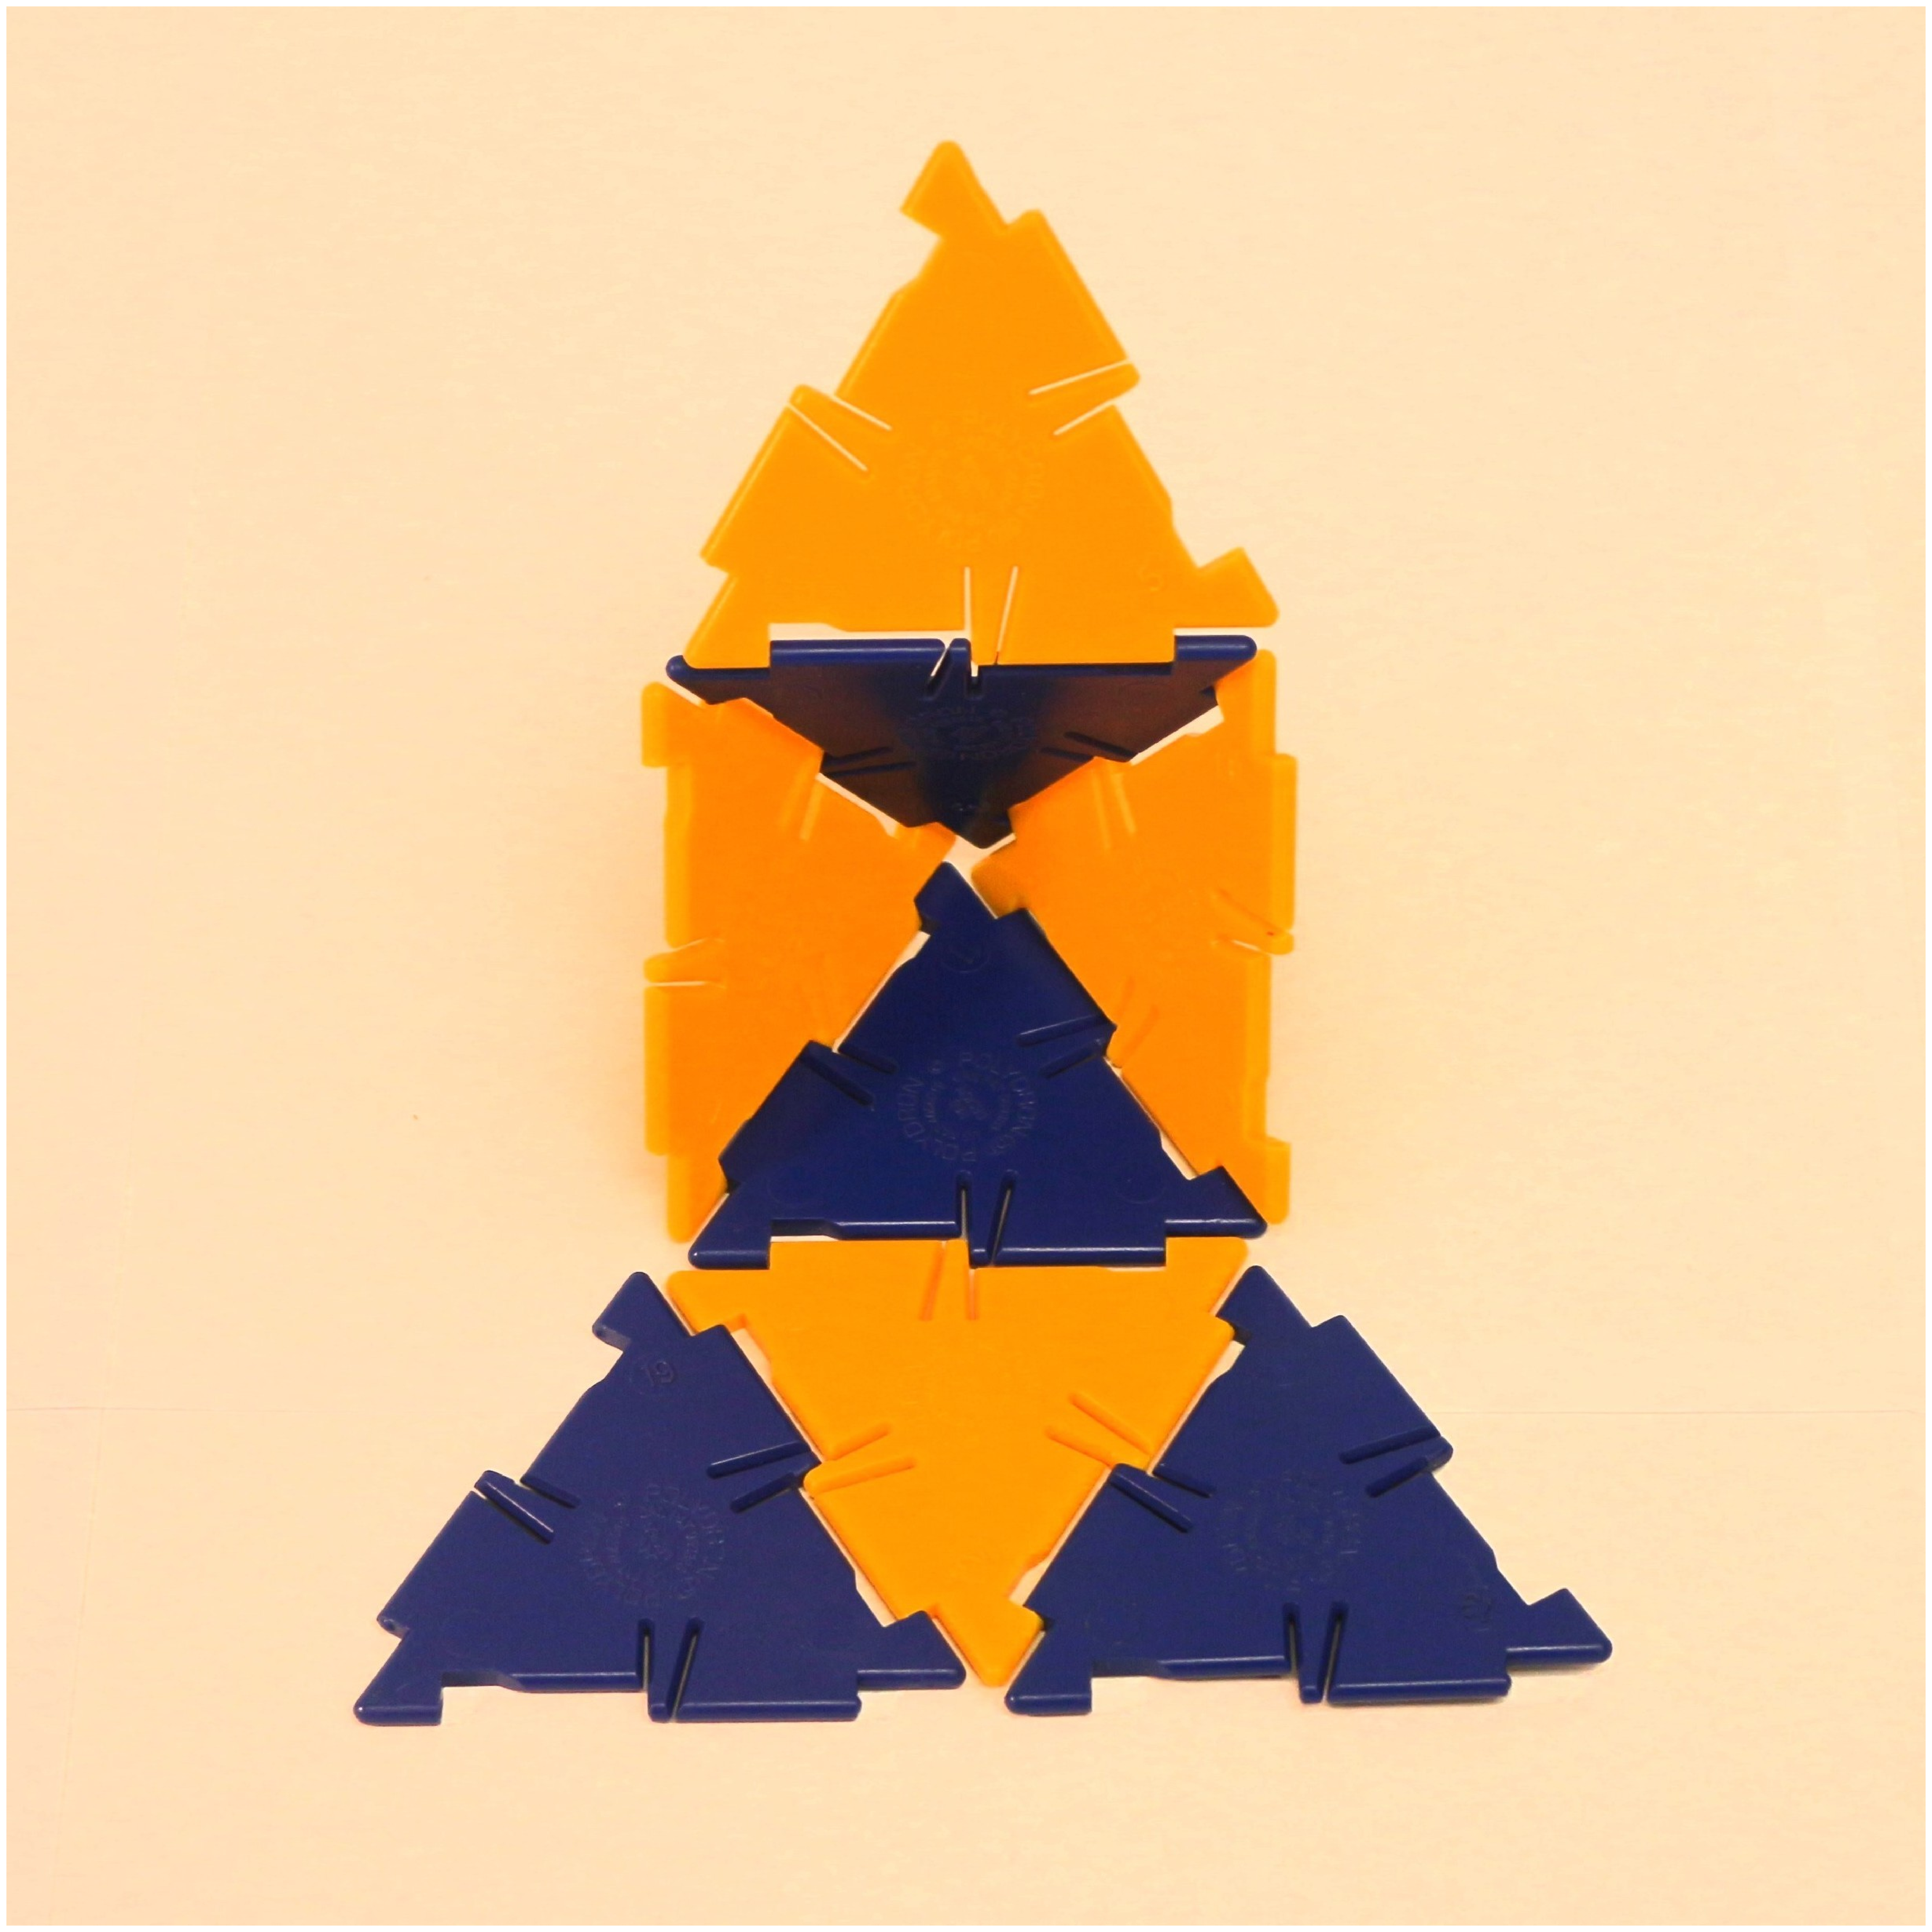
\includegraphics[width=0.18\textwidth]{images/folds_1.eps}
                
\includegraphics[width=0.18\textwidth]{images/folds_2.eps}
                
\includegraphics[width=0.18\textwidth]{images/folds_3B.eps}
                
\includegraphics[width=0.18\textwidth]{images/folds_4B.eps}


\caption{A sequence of Folding Model intermediates beginning with an octahedron net and resulting in the boat configuration.}
\label{fig:fold_boat}
\end{figure}

As a feature, this model has been shown to allow folds that do not result in the initially intended polyhedron and can terminate in other polyhedra and blocked states. For example, many of the intermediates that cannot fold into the octahedron end up folding into a non-convex boat intermediate. This is depicted in figure~\ref{fig:fold_boat}.

%Like in the Building Game, the state space of the folding model experiences a combinatorial explosion as the number of faces the polyhedron has increases. 

%\begin{mythm}
%Given a polyhedron $\mathcal{P}$, there exists a second polyhedron $\mathcal{P}'$ such that the sub-graph of folding state space containing intermediates that can still fold into $\mathcal{P}$ can be recovered from the Building Game state space for $\mathcal{P}'$.  
%\end{mythm}


\subsection{Local Rules}

A large number of previously studied models for self-assembly can be classifies as \textit{local rules} based approaches. Such models typically consist of a collection of components that can be combined according to a specified grammar. While this is a basic idea, the variety off possible component and grammars makes this a widely flexible class of models. Schwartz et al used such a model to describe the assembly of viral capsids~\cite{Berger1994, Schwartz1998}. Since these capsids are fundamentally composed of proteins that can each assume a number of conformations. By putting a grammar on the ways in which proteins of different conformation can combine, they were able to successfully form a variety of viral capsids in simulation. While this class of models is powerful, we have not actively pursued any such models. Introducing a local rules approach might allow the Building Game to be generalized in a way that allows formation errors as in the Folding Model.    


\subsection{Energy Landscapes}


%We first define a Markov Chain on the Building Game state space and identify the corresponding stationary distribution. 
%
%Associated with each intermediate $x_j$, we have the the combinatorial statistic $E_j \doteq -E(x_j)$ which is negative one times the number of edges in $x_j$ at which two faces meet. Thus, $E_k-E_j$ represents the number of such edges added (or removed) when a face is added to (or removed from) $x_j$ to form $x_k$. This statistic $E_j$ is an idealization of a bond energy within an intermediate.
%
%We define the Markov chain $X_t$ by the transition rule $P_{jk} \doteq P(X_{t+1} = x_k | X_t = x_j)$, with the heuristic that it should be more likely for an intermediate to add a face in a location in which more new edge connections can be formed.
%
%% \begin{numcases}{P_{jk} =}
%%        \frac{1}{z_j}s_{j,k}e^{-\frac{1}{2}\beta\left(E_k-E_j\right)}  & $j \neq k, j \leftrightarrow k$ \\
%%        \frac{1}{z_j}\phi_j \label{eq:A} & $j = k$\\
%%        0 & $j \neq k, j \not\leftrightarrow k$
%%        \end{numcases}
%
%$$
% P_{jk} = \begin{cases}
%        \frac{1}{z_j}S_{j,k}e^{-\frac{1}{2}\beta\left(E_k-E_j\right)}  & j \neq k, j \leftrightarrow k \\
%        \frac{1}{z_j}\phi_j \label{eq:A} & j = k\\
%        0 & j \neq k, j \not\leftrightarrow k 
%       \end{cases}
%$$
%Here the self-transition likelihoods $\left\{\phi_j\right\}$ and the thermodynamic $\beta$, are parameters that can be chosen later. We define the normalization constants as $z_j \doteq \phi_j + \sum_{k\neq j}S_{jk}e^{-\beta\left(E_k-E_j\right)}\mathbb{1}_{j\leftrightarrow k}$. 
%
%
%Since we define Building Game intermediates as rotationally unique from each other, it is useful to think about the rotational symmetry group of each intermediate. For an intermediate $x_j$, we define $r_j$ to be the order of the rotation group of $x_j$. By polyhedral group theory arguments, we have proven the following theorem.
%\begin{mythm}
%\label{thm:C}
%For two Building Game intermediates $x_j$ and $x_k$ connected in the BG state space, $r_j = S_{jk}C_{jk}$.
%\end{mythm}
%While we indeed have a precise geometric definition of the values $C_{jk}$, it is most important to not that $C_{jk} = C_{kj}$ is symmetric. This symmetry is useful since the degeneracy number $S_{jk}$ is not itself symmetric in general. By assuming detailed balance, theorem~\ref{thm:C} allows us to derive a stationary distribution for $X_t$.
%\begin{mythm}
%The Markov chain $X_t$ defined by the transition rule $P_{jk}$ admits the unique stationary distribution $\pi_j = \frac{1}{z}\left(\frac{z_j}{r_j}\right)e^{-\beta E_j}$. 
%\end{mythm}
%
%One way to define the concept of a dominant intermediate or pathway is with respect to this stationary distribution. However, dynamics should not be overlooked. One natural question to ask is: which pathway has the highest probability of occurring with respect to our transition probabilities? More formally, we can put a probability on a pathway $x_0 = x_{n_1},x_{n_2},x_{n_3},...,x_{n_F}=x_F$ as the following product. 
%$$P\left(x_{n_1},x_{n_2},x_{n_3},...,x_{n_F}\right) \doteq \prod_{k=1}^F P_{n_{k-1}n_k} \propto \prod^F_{k=1}S_{n_{k-1}n_k}$$
%Of course, this definition does not allow for backward transitions which can play an important role in the correction of less favorable intermediates, but it provides a probabilistically motivated heuristic. 
%
%Since we are interested in the formation of the completed polyhedron beginning from a single face, we can ask about how likely a specific intermediate is to be reached if the state transitions until it reaches the terminal closed polyhedron. If we define the stopping time $\tau_k \doteq \inf\left\{n>0: X_n = x_k\right\}$ with $\tau_F$ the equivalent stopping time corresponding to the terminal state, we can formulate this question as computing the probability $\rho_k\left(\beta\right) \doteq P\left(\tau_k < \tau_F\right)$. These statistics can be computed exactly via dynamic programming, but it is possible that martingales or other analytic tools would allow a more direct and illuminating derivation. 
%

Due to the scale of many of these self-assembly processes, statistical mechanics provides a framework to think about these models. By finding an analogy with a diffusion process on an implied potential energy surface, we can use statistical mechanical tools to examine the properties of this potential surface. 

Reversible Markov processes can be used for a variety of different discrete models for self-assembly. If a graph of the model's possible configurations is known, one can put a Markov process on this graph as a discrete version of a diffusion process on an energy landscape. By giving each graph node an energy level and treating graph edges as barriers, the Markov process transition rates are related to the height of the energy barrier that must be overcome to jump to another node. With this flexible mathematical machinery, a wide variety of questions can be asked: from pathway probabilities to formation related stopping times.

%The folding model tends to describe an irreversible process, so some of the concepts inherent to reversible Markov processes, such as the stationary distribution would not apply. The dynamical aspects, however, may still be appropriately modeled with Markov processes. While we have not explored the topic extensively, it seems as though, due to their modeling and analytic flexibility, Markov processes provide a natural approach to many local rules type models as well. 


\subsection{Disconnectivity Graphs and Qualitative Approaches}

Wales et al. introduced a graphical way to represent the structure of a potential surface possessing many local minima and intermediary transition states~\cite{Wales1998, Doye1999}. Named a \textit{discontinuity graph}, the tree with leaves representing local minima of the potential and other connecting nodes representing transition states that the minima can be reached from provides a way of picturing the structure of the a potentially high dimensional energy landscape that looks past simple energy differences. The vertical height of each node is used to represent the potential energy of that state. Horizontally, the tree is organized to partition these local minima into corresponding funnels. If the graph is truncated at a specific energy level, two minima are reachable via transitions to states strictly below this truncation energy if and only if they remain connected in the truncated disconnectivity tree. 

%\begin{figure}[!h]
%%\centering
%%\includegraphics[width=0.5\textwidth]{Wales_DG_LJ.png}
%\caption{Example of disconnectivity tree.}%A disconnectivity tree for the 38-atom Lennard-Jones cluster. [from Wales et al]} -- Can use???
%\label{fig:dg}
%\end{figure}

%Depicted in figure~\ref{fig:dg} is the disconnectivity graph for a 38-atom Lennard-Jones cluster. This DG is described as having two funnels since there are two low energy local minima (one of which is the global minimum) that are far from each other in the graph and yet not of significantly different energy levels. This suggests that the cluster could be energetically trapped in the non-global minima and it would take a prohibitive amount of time to escape to the global minimum. 

While not a quantitative way of assessing a model's pathways, disconnectivity graphs are extremely useful in identifying broad qualitative properties and can be instrumental in gaining insight into a model's dynamics. The use of such graphical and otherwise qualitative techniques should not be overlooked as they can inspire techniques for more quantitative analysis.  

%\section{Prior Work}
%
%While models such as the Building Game treat assembly intermediates as idealized structures, the intermediates of the physical application we are trying to model may face a chaotic and volatile range of forces. To more realistically model the ways in which our intermediate might flex and move under these forces, we impose a constraint model in with the rigidity of individual components of an intermediate are assumed, but in which the edges at which they meet are treated like a hinge. This constraint system specifies the ways in which an intermediate has freedom to move if it is able to move at all. A physically motivated way of addressing questions that the discrete models themselves are not adequate to answer is provided by this framework.   
%
%\subsection{Configuration Space}
%
%To characterize the freedoms of three-dimensional intermediates composed of rigid two-dimensional faces and connected at hinged edges, we parameterize each face and impose constraints in parameter space. Theoretically, the location and orientation of each face of an intermediate can be parameterized by six parameters: three for translation, three for rotation. This means the configuration of the entire intermediate can be represented by at most $6|F|$ parameters. In practice, however, it is often advantageous for ease of analysis and computational implementation to use more parameters to represent a given configuration. Often times, we use $3$ parameters to represent the location each vertex of each face, even if some of these vertices share common locations. This means that we often have an ambient parameter space of $\mathbb{R}^N$ with $N > 6|F|$. 
%
%Upon this parameter space we place three types of constraints. The first removes the configuration's 6 trivial degrees of freedom due to translation and rotation. Since the intermediate is connected, this can be achieved by fixing the parameters of one of the intermediate's faces. Additionally, we enforce a rigidity constraint on each face ensuring that the structure of a constituent face will not change with movement of the larger structure. The final type of constraint ensures that the connections between two faces have hinge-like mobility. Since a shared edge has two vertices belonging to each face, this constraint is imposed by identifying the corresponding vertex locations. 
%
%The \textit{configuration space} is defined to be the subset of ambient space $\left\{z \in \mathbb{R}^N : \varphi\left(z\right) = 0\right\}$  for which all $M$ of the constraint equations $\varphi: \mathbb{R}^N \to  \mathbb{R}^M $ are satisfied.  Since it is assumed that the standard configuration of the intermediate given by the model satisfies the constraints, the configuration space is non-empty. The configuration space is an algebraic variety, because the constraint equations can typically be represented as (quadratic) polynomials.  The \textit{degrees of freedom} of a particular configuration is taken to be the dimension of the null space of the Jacobian of $\varphi$. This is due to the fact that any move in the ambient space that prevents the constraint equations from changing must also be in the configuration space. Interestingly, it is possible for some members of configuration space to have a different number of degrees of freedom than others. 
% 
%It is important to note that there are many possible parameterizations of a configuration and the choice of which will likely result in a different configuration space. The selection of which face to constrain in order to remove the trivial degrees of freedom may also affect the structure of the configuration space. While we must be cognizant of these choices, in many cases, the properties we wish to evaluate of the configuration space are independent of the choices.
%
%%\subsection{Cyclohexane}
%%
%%One example of using the 
%%
%\subsection{Constrained Dynamics}
%
%Sometimes we are interested in more that simply the number of degrees of freedom a particular configuration has. To explore the configuration space, find connections between different admissible configurations, analyze the configuration space's topology, or compute other relevant statistics, it can be useful to compute dynamics on the constraint space. There are clear computational challenges to computing such dynamics due to the fact that configuration space is often of much smaller dimension than the ambient space it sits in. 
%
%Constraint algorithms have been widely studied for use in molecular dynamic simulations: we use the SHAKE algorithm and application specific variants. The SHAKE algorithm is a two stage method in which the laws of motion are first used to evolve the system to an unconstrained configuration $\hat{y}_{n+1}$ based on the previous configuration $y_n$. In the second stage, Lagrange multipliers are used to correct $\hat{y}_{n+1}$ to a new configuration $y_{n+1}$ which satisfies the constraints. 
%
%Assuming connectedness of the configuration space, constraint algorithms can be used to compute various statistics of the configuration space. For example, the $d$-dimensional volume of a $d$-dimensional configuration space can be used to measure how much mobility the intermediate has in its configuration space. Additionally, if we have soft constraints, such as preferred angles between faces, we can institute cost functions on the configuration space with configurations having more favorable angles having a lower cost. Whether physically or artificially motivated, such cost functions can be treated as potential energy functions which can imply specific dynamics. Under this set of dynamics, quantities such as the average or minimum energies may be of interest. 
%
%We may also be interested in the behavior of a small part of the configuration as it undergoes constrained dynamics. For instance, suppose we are interested in the tendency for two edges on distinct faces to come together and form a new connection. By looking at the distance between these edges, we can measure how frequently this event happens and the probability that it will occur before another even of interest. This is similar to the exit time problem for diffusion and may provide a physically motivated evaluation tool for the appropriateness of our transition rules we adopt in our models. 
%
\section{Original Contributions}


As the Building Game was previously studied as a tool for modeling chemical processes, we have added mathematical formalisms that we not previously relevant. In particular, using the theory of group actions has allowed a more in-depth conversation about the role of symmetry in the Building Game and self-assembly processes in general.

By enumerating the combinatorial configuration space for all Platonic, Archimedean, and Catalan solids up to 30 faces, a foundation is set for later analyses. As part of this enumeration work, previously unknown combinatorial statistics of these polyhedra were derived. Of particular importance is the calculation of the number of shellings each polyhedron has.  

Our use of hinged polygonal linkages to model the internal mobility of a partially assembled polyhedron adds a geometric perspective to the Building Game on top of the existing combinatorial structure. Using constraint equations to mathematically describe the geometric configurations that such linkages can take allowed us to compute the number of degrees of freedom of Building Game intermediates. To examine additional properties of Building Game geometric configuration spaces, a reflected Brownian motion on implicitly defined constraint spaces was considered. By developing a corresponding manifold reflected random walk scheme, we sampled geometric configurations.



%-- Counted degrees of freedom of BG intermediates.

%-- Developed a manifold reflected Brownian motion scheme to sample configurations.


%-- Used energetic perspective to model BG processes as a reversible Markov chain.


Our most important contributions lie in the combination of combinatorial and geometric aspects of the Building Game model for self-assembly. By taking an energetic perspective, a reversible Markov chain was defined on the Building Game configuration space with transition rates informed by the reflected Brownian motion simulated in the geometric configuration space for each intermediate. 

%-- Formalized mathematical framework for BG
%-- Enumerated combinatorial configuration space for all Platonic, Archimedean, and Catalan solids up to 30 faces.
%-- First to enumerate the number of shellings of these polyhedral classes.
